\documentclass[a4paper,12pt]{report}

\usepackage{cmap}
\usepackage[T2A]{fontenc}
\usepackage[utf8]{inputenc}
\usepackage[english,russian]{babel}
\usepackage{listings}
\usepackage{amsmath}
\usepackage{float}
\usepackage{csquotes}
\usepackage{mathtools}

\usepackage{xcolor}
\usepackage{hyperref}

\usepackage{graphicx}
\graphicspath{ {./img/} }

\definecolor{dkgreen}{rgb}{0,0.6,0}
\definecolor{gray}{rgb}{0.5,0.5,0.5}
\definecolor{mauve}{rgb}{0.58,0,0.82}

\lstset{
    language=Python,                
    basicstyle=\small\sffamily, 
    numbers=left,               
    numberstyle=\tiny,           
    stepnumber=1,                   
    numbersep=5pt,                
    aboveskip=3mm,
    belowskip=3mm,
    showstringspaces=false,
    columns=flexible,
    captionpos=b, 
    basicstyle={\small\ttfamily},
    numbers=left,
    numberstyle=\tiny\color{gray},
    keywordstyle=\color{blue},
    commentstyle=\color{mauve},
    stringstyle=\color{dkgreen},
    breaklines=true,
    breakatwhitespace=true,
    tabsize=3
}

\title{Лабораторная работа №2\\Гармоники}
\author{Крынский Павел}
\date{\today}

\begin{document}

\maketitle
\tableofcontents
\listoffigures
\lstlistoflistings

\maketitle

\chapter{Упражнение 2.1}

В данном упражнении нас просят открыть \texttt{chap02.ipynb}, прочитать пояснения и запустить примеры. Поэтому здесь я изучил все примеры с комментариями и позапускал их.

\chapter{Упражнение 2.2}
\section{Написание класса и проверка сигнала}

Для данного упражнения нужно написать класс под названием \texttt{SawtoothSignal} и за основу просят взять \texttt{Signal}, но в главе примеры на основе \texttt{Sinusoid}, поэтому я буду использовать \texttt{Sinusoid}.

\begin{lstlisting}[caption=Класс SawtoothSignal]
class SawtoothSignal(thinkdsp.Sinusoid):
    def evaluate(self,ts):
        cycles = self.freq * ts + self.offset / thinkdsp.PI2
        frac , _ = np.modf(cycles)
        ss = self.amp * frac
        return ss
\end{lstlisting}

Убедимся, что все работает корректно.

\begin{lstlisting}[caption=Визуализация пилообразного звука]
ss = SawtoothSignal()
ss_wave = ss.make_wave(ss.period*3 , framerate = 20000)
ss_wave.plot()
\end{lstlisting}

\begin{figure}[H]
        \centering
        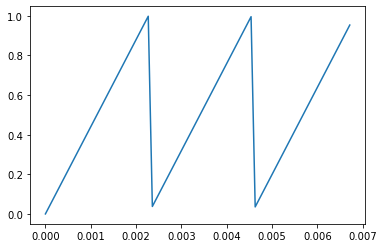
\includegraphics[width=0.75\textwidth]{1.png}
        \caption{Полученный пилообразный звук}
        \label{fig:fig2_1}
\end{figure}
    


\section{Спектр звука}

Теперь рассмотрим спектр нашего пилообразного звука.

\begin{lstlisting}[caption=Спектр звука]
spectr = ss_wave.make_spectrum()
spectr.plot()
\end{lstlisting}

\begin{figure}[H]
        \centering
        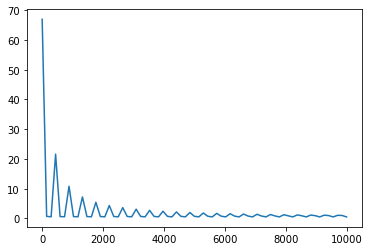
\includegraphics[width=0.75\textwidth]{2.png}
        \caption{Спектр сегмента звука}
        \label{fig:fig2_2}
\end{figure}

В сравнении с треугольной волной пилообразная форма уменьшается практически аналогично, но включает как четные, так и нечетные гармоники.


\chapter{Упражнение 2.3}

Нам нужно создать прямоугольный сигнал 1100 Гц и вычислить его спектр.
Создадим прямоугольный сигнал 1100 Гц и вычислим его спектр.

\begin{lstlisting}[caption=Создание прямоугольного сигнала]
signal = thinkdsp.SquareSignal(1100)
wave = signal.make_wave(duration=0.5, framerate=10000)
spectr = wave.make_spectrum()
spectr.plot()
\end{lstlisting}

\begin{figure}[H]
        \centering
        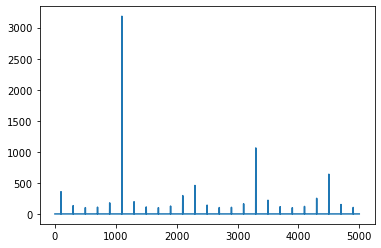
\includegraphics[width=0.75\textwidth]{3.png}
        \caption{Спектр сегмента звука}
        \label{fig:fig3_1}
\end{figure}

Основная и первая гармоника находятся в нужном месте, но вторая гармоника, которая должна быть 5500 Гц, смещается на 4500 Гц. Третья, которая должна быть 7700 Гц, находится на 2300 Гц и так далее. Прослушаем полученный звук.

\begin{lstlisting}[caption=Воспроизведение прямоугольного сигнала]
wave.make_audio()
\end{lstlisting}

Когда мы слушаем полученную волну, можем слышать эти aliasing-гармоники, поскольку низкий тон имеет частоту 300 Гц. Создадим такой сигнал и прослушаем его. Разница присутствует и данные частоты можно расслышать.

\begin{lstlisting}[caption=Создание и воспроизведение сигнала с пониженной частотой]
thinkdsp.SinSignal(300).make_wave(duration=0.5, framerate=10000).make_audio()
\end{lstlisting}

\chapter{Упражнение 2.4}
\section{Создание сигнала}

Создадим треугольный сигнал с частотой 440 Гц и \texttt{wave} длительностью 0,01 секунды.

\begin{lstlisting}[caption=Создание треугольного сигнала]
signal = thinkdsp.TriangleSignal()
wave = signal.make_wave(duration=0.01)
wave.plot()
\end{lstlisting}

\begin{figure}[H]
        \centering
        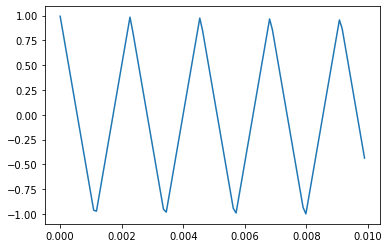
\includegraphics[width=0.75\textwidth]{4.png}
        \caption{Визуализация созданного сигнала}
        \label{fig:ig4_1}
\end{figure}

\section{Нулевой компонент спектра}

Первый элемент спектра - комплексное число, близкое к нулю. Если мы добавим в компонент нулевой частоты какое-то число, то это приведет к добавлению вертикального смещения спектра.

\begin{lstlisting}[caption=Вывод нулевого компонента]
spectr = wave.make_spectrum()
spectr.hs[0]
\end{lstlisting}

На выходе получили \texttt{(1.0436096431476471e-14+0j)}.

\section{Изменение нулевого компонента}

Теперь установим смещение равное 100 и увидим, что сигнал сместился по вертикали.

\begin{lstlisting}[caption=Смещение спектра и его визуализация]
spectr.hs[0] = 100
spectr.make_wave().plot()
\end{lstlisting}

\begin{figure}[H]
        \centering
        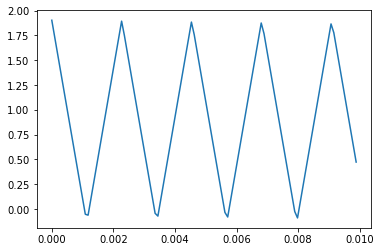
\includegraphics[width=0.75\textwidth]{5.png}
        \caption{Визуализация ускоренного звука}
        \label{fig:fig4_2}
\end{figure}

\chapter{Упражнение 2.5}
\section{Создание функции}

Напишем функцию, которая принимает \texttt{Spectrum} в качестве парметра и иизменяет его делением каждого элемента \texttt{hs} на соответсвующую частоту из \texttt{fs}.

\begin{lstlisting}[caption=Создание функции]
def modif(spectr):
    for it in range (1 , len(spectr.hs)):
        spectr.hs[it] = spectr.hs[it] / spectr.fs[it]
    spectr.hs[0] = 0
\end{lstlisting}

\section{Проверка работоспособности функции}

Создадим прямоугольный сигнал и прослушаем его.

\begin{lstlisting}[caption=Создание сигнала и его воспроизведение]
wave = thinkdsp.SquareSignal(freq=400).make_wave(duration = 0.5)
wave.make_audio()
\end{lstlisting}

Теперь выведем только что созданный спектр, а также изменим его при помощи нашей функции и посмотрим на результат.

\begin{lstlisting}[caption=Сравнение спектров]
spectrum = wave.make_spectrum()
spectrum.plot(high = 10000 ,color = 'red' )
modif(spectrum)
spectrum.scale(400)
spectrum.plot(high = 10000 )
\end{lstlisting}

\begin{figure}[H]
        \centering
        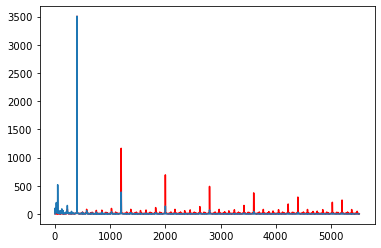
\includegraphics[width=0.75\textwidth]{6.png}
        \caption{Сравнение спектров}
        \label{fig:fig5_1}
\end{figure}

Фильтр подавляет гармоники, поэтому он действует как фильтр низких частот. Звук слышется почти как синусоида.

\begin{lstlisting}[caption=Воспроизведение отфильтрованного звука]
sp = spectrum.make_wave()
sp.make_audio()
\end{lstlisting}

\chapter{Упражнение 2.6}

Создадим пилообразный сигнал и выведем его спектр.

\begin{lstlisting}[caption=Создание сигнала и визуализация его спектра]
signal = thinkdsp.SawtoothSignal(freq=500)
wave = signal.make_wave(duration=0.5, framerate=20000)
wave.make_audio()
spectr = wave.make_spectrum()
spectr.plot()
\end{lstlisting}

\begin{figure}[H]
        \centering
        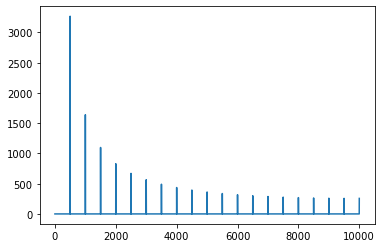
\includegraphics[width=0.75\textwidth]{7.png}
        \caption{Спектр сигнала}
        \label{fig:fig6_1}
\end{figure}

На рисунке видно, что гармоники уменьшаются как \(1 / f\).

\begin{lstlisting}[caption=Сравнение гармоник]
spectr.plot(color='red')
modif(spectr)
spectr.scale(500)
spectr.plot()
\end{lstlisting}

\begin{figure}[H]
        \centering
        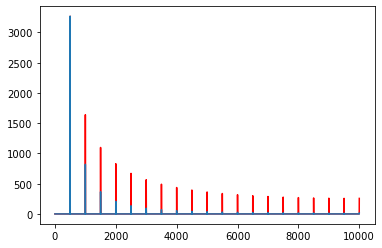
\includegraphics[width=0.75\textwidth]{8.png}
        \caption{Спектр сигнала}
        \label{fig:fig6_2}
\end{figure}

Теперь гармоника схожа с синусоидой.

\begin{lstlisting}[caption=Сегмент звука]
wave.segment(duration=0.01).plot()
\end{lstlisting}

\begin{figure}[H]
        \centering
        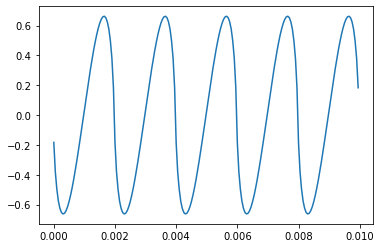
\includegraphics[width=0.75\textwidth]{9.png}
        \caption{Сравнение спектров}
        \label{fig:fig6_3}
\end{figure}

\chapter{Выводы}

Во время выполнения лабораторной работы получены навыки работы с новыми сигналами и их гармониками, а именно с треугольными, прямоугольными и пилообразными сигналами. Также рассмотрено одно из наиболее важных явлений в цифровой обработке сигналов - биения.

\end{document}